%!TEX program = xelatex
\documentclass[10pt, compress, handout]{beamer}
\usepackage[titleprogressbar]{../../cls/beamerthemem}

\setbeamertemplate{caption}[numbered]
\setbeamertemplate{theorems}[numbered]
\newcounter{example}
\resetcounteronoverlays{example}
\newtheorem{crl}{Corollary}[theorem]
\newtheorem{eg}[example]{Example}
\newtheorem*{solution*}{Solution}

\usepackage{booktabs}
\usepackage[scale=2]{ccicons}
\usepackage{minted}

\usepackage{cleveref}
\crefname{example}{Example}{Examples}

\usepgfplotslibrary{dateplot}

\usemintedstyle{trac}

\usepackage{algorithm}
\usepackage[noend]{algpseudocode}
\resetcounteronoverlays{algorithm}

\usepackage[linguistics]{forest}
\usepackage{listings}
\usepackage{mathtools}
\usepackage{multicol}
\usepackage{qtree}

\usepackage{tikz}

\usepackage{version}
% \excludeversion{proof}
% \excludeversion{solution*}

\makeatletter
\def\old@comma{,}
\catcode`\,=13
\def,{%
    \ifmmode%
    \old@comma\discretionary{}{}{}%
    \else%
    \old@comma%
    \fi%
}
\makeatother

\title{CENG 4120 Tutorial of Week 10}
\subtitle{Mid-Term}
\author{LI Haocheng}
\institute{Department of Computer Science and Engineering}

\begin{document}

\maketitle

\begin{frame}
\frametitle{Complementation}
\begin{eg}
    Prove that $(\overline{F})_x = \overline{F_x}$.
\end{eg}
\onslide<2->\begin{proof}
    We can divide the SOP terms of $F$ in three categories: $F = xF_+ + \overline{x}F_- + F_0$ where $xF_+$ equals all terms with $x$, $\overline{x}F_-$ equals all terms with $\overline{x}$ and $F_0$ equals all terms without $x$ or $\overline{x}$ then we have $F_{x = 1} = F_+ + F_0$ and $F_{x = 0} = F_- + F_0$.
    Therefore, \begin{align}
    \begin{aligned}
    \overline{F_x} = & \overline{xF_{x = 1} + \overline{x}F_{x = 0}}\\
    = & \overline{x (F_+ + F_0) + \overline{x}(F_- + F_0)}\\
    = & (\overline{x} + \overline{(F_+ + F_0)})(x + \overline{(F_- + F_0)})\\
    = & x\overline{(F_+ + F_0)} + \overline{x}\overline{(F_- + F_0)}\\
    = & x\overline{F}_{x = 1} + \overline{x}\overline{F}_{x = 0} = \left(\overline{F}\right)_x.
    \end{aligned}
    \end{align}
\end{proof}
\end{frame}

\begin{frame}
\frametitle{Or}
\begin{eg}
    Prove that $(F + G)_x = F_x + G_x$.
\end{eg}
\onslide<2->\begin{proof}
    Let $F = xF_+ + \overline{x}F_- + F_0$ and $G = xG_+ + \overline{x}G_- + G_0$, where any of $F_+, F_-, F_0, G_+, G_-, G_0$ is not supported by $x$, then $F + G = x(F_+ + G_+) + \overline{x}(F_- + G_-) + F_0 + G_0$.
    \begin{align}
    \begin{aligned}
    F_x + G_x = & xF_{x = 1} + \overline{x}F_{x = 0} + xG_{x = 1} + \overline{x}G_{x = 0}\\
    = & x(F_+ + F_0) + \overline{x}(F_- + F_0)+ x(G_+ + G_0) + \overline{x}(G_- + G_0)\\
    = & x(F_+ + G_+ + F_0 + G_0) + \overline{x}(F_- + G_- + F_0 + G_0)\\
    = & x(F + G)_{x = 1} + \overline{x}(F + G)_{x = 0}\\
    = & \left(F + G\right)_x.
    \end{aligned}
    \end{align}
\end{proof}
\end{frame}

\begin{frame}
\frametitle{And}
\begin{eg}
    \label{eg:shannon}
    Prove that \begin{enumerate}
        \item $(F \cdot G)_x = F_x \cdot G_x$.
        \item $(F \oplus G)_x = F_x \oplus G_x$.
    \end{enumerate}
\end{eg}
\begin{proof}
    \begin{enumerate}
        \item<2->\begin{align}
        \begin{aligned}
        (F \cdot G)_x = & x (F \cdot G)_{x = 1} + \overline{x} (F \cdot G)_{x = 0} = x F_{x = 1} G_{x = 1} + \overline{x} F_{x = 0} G_{x = 0}\\
        = & x F_{x = 1} x G_{x = 1} + x F_{x = 1} \overline{x} G_{x = 0} + \overline{x} F_{x = 0} x G_{x = 1} + \overline{x} F_{x = 0} \overline{x} G_{x = 0}\\
        = & (x F_{x = 1} + \overline{x} F_{x = 0}) \cdot (x G_{x = 1} + \overline{x} G_{x = 0}) = F_x \cdot G_x.
        \end{aligned}
        \end{align}
        \item<3> \begin{align}
        \begin{aligned}
        (F \oplus G)_x = & (\overline{F}G + F\overline{G})_x = (\overline{F}G)_x + (F\overline{G})_x = (\overline{F})_x G_x + F_x (\overline{G})_x\\
        = & \overline{F_x} G_x + F_x \overline{G_x} = F_x \oplus G_x.
        \end{aligned}
        \end{align}
    \end{enumerate}
\end{proof}
\end{frame}

\begin{frame}[fragile]
\frametitle{Circuit Repair}
\begin{columns}
    \column{.7\linewidth}
    \begin{eg}
        Suppose a circuit has a mal-functioned OR gate.
        \begin{figure}
            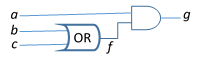
\includegraphics[width=.4\linewidth]{image_2019-03-12_21-26-14}
            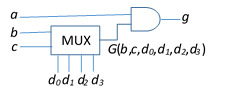
\includegraphics[width=.4\linewidth]{image_2019-03-12_21-32-54}
            \caption{Mal-functioned Circuit}
        \end{figure}
    \begin{enumerate}
        \item Construct the function $G(b, c, d_0, d_1, d_2, d_3)$.
        \item Construct a function $Z(b, c, d_0, d_1, d_2, d_3)$ such that $Z \equiv 1$
        if and only if $G \equiv (b + c)$
        \item Show how to derive the four inputs $d_0$, $d_1$, $d_2$, $d_3$ to the MUX using the quantification operator on $Z$.
    \end{enumerate}
    \end{eg}

\column{.4\linewidth}
\begin{solution*}
    \begin{enumerate}
        \item<2-> $G = d_0 \overline{b} \overline{c} + d_1 \overline{b}c + d_2 b \overline{c} + d_3 b c$.
        \item<3-> $Z = G \odot (b + c)$.
        \item<4> We have $\forall b, c ~ Z = 1$. Then $Z_{b = 0, c = 0} \cdot Z_{b = 0, c = 1} \cdot Z_{b = 1, c = 0} \cdot Z_{b = 1, c = 1} = 1$. Therefore $d_0 = 1 \odot 0 = 0$, $d_1 = 1 \odot 1 = 1$, $d_2 = 1 \odot 1 = 1$, $d_3 = 1 \odot 1 = 1$.
    \end{enumerate}
\end{solution*}
\end{columns}
\end{frame}

\begin{frame}[fragile]
\frametitle{PCN}
\begin{columns}
    \column{.6\linewidth}
    \onslide<1->\begin{eg}
        \begin{figure}
            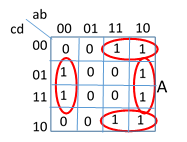
\includegraphics[width=.4\linewidth]{image_2019-03-12_22-23-02}
            \caption{K-Map of $F$}
        \end{figure}
    \begin{enumerate}
        \item PCN cube list of $F$.
        \item PCN cube list of $F'$.
        \item Expand $A$ maximally. Revise the PCN cube list in (i) to reflect this expansion.
    \end{enumerate}
    \end{eg}
\column{.5\linewidth}
    \begin{solution*}
        \begin{enumerate}
            \item<2-> $F = a \overline{b} d + a \overline{c} \overline{d} + ac \overline{d} + \overline{a} \overline{b} d$.
            \item<3-> $F' = bd + \overline{a} \overline{d}$.
            \item<4> The blocking matrix is shown as follows.
            \begin{table}
                \begin{tabular}{c|cc}
                & $bd$ & $\overline{a} \overline{d}$\\\midrule
                $a$ & & $1$\\
                $\overline{b}$ & $1$ &\\
                $d$ & & $1$
            \end{tabular}
        \caption{Blocking Matrix}
            \end{table}
        
        $F = \overline{b} d + a \overline{c} \overline{d} + ac \overline{d} + \overline{a} \overline{b} d$.
        \end{enumerate}
    \end{solution*}
\end{columns}
\end{frame}

\begin{frame}[fragile]
\frametitle{Kernel}
\begin{columns}
    \column{.3\linewidth}
    \onslide<1->\begin{eg}
        Consider the following Boolean function $F = ac'd'e' + acd'e + bde + bce + abc'$, $G = bc'de + d'e'$.
        \begin{enumerate}
            \item Rewrite F and G.
            \item Find all the kernels and co-kernels of F, using the recursive algorithm \texttt{FindKernels()}.
        \end{enumerate}
    \end{eg}

\column{.8\linewidth}
\begin{solution*}
    \begin{enumerate}
        \item<2-> Let $f = c'$, $g = d'$, $h = e'$. Then we have $F = afgh + acge + bde + bce + abf$ and $G = bfde + gh$.
        \item<3> \hspace{-.4in}\resizebox{1.1\linewidth}{!}{\begin{forest}
            [$afgh + acge + bde + bce + abf$[$\begin{matrix}
            \mathrm{cubes} & afgh + acge + abf\\
            \mathrm{co} & a\\
            \mathrm{kernel} & fgh + cge + bf
            \end{matrix}$[$\begin{matrix}
            \mathrm{cubes} & fgh + bf\\
            \mathrm{co} & f\\
            \mathrm{kernel} & gh + b
            \end{matrix}$[no work]][$\begin{matrix}
            fgh + cge\\
            g\\
            fh + ce
            \end{matrix}$[no work]]][$\begin{matrix}
            bde + bce + abf\\
            b\\
            de + ce + af
            \end{matrix}$[$\begin{matrix}
            de + ce\\
            e\\
            c + d
            \end{matrix}$[no work]]][$\begin{matrix}
            acge + bce\\
            ce\\
            ag + b
            \end{matrix}$[no work]][$\begin{matrix}
            acge + bde + bce\\
            e\\
            acg + bd + bc
            \end{matrix}$[$\begin{matrix}
            bd + bc\\
            b\\
            c + d
            \end{matrix}$[no work]][$\begin{matrix}
            acg + bc\\
            c\\
            ag+ b
            \end{matrix}$[no work]]][$\begin{matrix}
            afgh + abf\\
            af\\
            gh + b
            \end{matrix}$[no work]][$\begin{matrix}
            afgh + acge\\
            ag\\
            fh + ace
            \end{matrix}$[no work]]]
        \end{forest}}
    
    \hspace{-.5in}\begin{tabular}{cc|cc}
        Kernel & Co& Kernel & Co\\\midrule
        $gh + b$ & $af$ & $de + ce + af$ & $b$\\
        $fh + ce$ & $ag$ & $ag + b$ & $ce$\\
        $fgh + cge + bf$ & $a$ & $acg + bd + bc$ & $e$\\
        $c + d$ & $be$ & $afgh + acge + bde + bce + abf$ & $1$
    \end{tabular}
    \end{enumerate}
\end{solution*}
\end{columns}
\end{frame}

\begin{frame}[fragile]
\frametitle{Kernel Level}
\begin{columns}
    \column{.5\linewidth}
    \onslide<1->\begin{eg}
        Modify \texttt{FindKernels()} to return just the level-0 kernels.
    \end{eg}
\onslide<2->\begin{solution*}
    \begin{algorithmic}
        \Procedure{FindKernels}{$f$}
        \State $K \coloneqq \emptyset$
        \For{$i \coloneqq 1 \cdots m$}
        \If{$\left|\Call{Cubes}{f, x_i}\right| \ge 2$}
        \State \textbf{continue}
        \EndIf
        \State $C \coloneqq \bigcap \Call{Cubes}{f, x_i}$
        \State $K \coloneqq K \cup \Call{Find}{f / C}$
        \EndFor
        \If{$K = \emptyset$} \Return $\{f\}$
        \Else ~ \Return $K$
        \EndIf
        \EndProcedure
    \end{algorithmic}
\end{solution*}
\column{.6\linewidth}
\onslide<1->\begin{eg}
    Draw a K-map for the Boolean function $Z = X \oplus Y \oplus b$. Obtain a SOP expression for $Z$ with the smallest number of literals.
\end{eg}
\onslide<3>\begin{solution*}
    \begin{table}
        \caption{Karnaugh Map}
        \begin{tabular}{c|cccc}
            $b$\textbackslash$XY$ & $00$ & $01$ & $11$ & $10$ \\\midrule
            $0$ & $0$ & $1$ & $0$ & $1$ \\
            $1$ & $1$ & $0$ & $1$ & $0$ \\
        \end{tabular}
    \end{table}

    \begin{equation}
        Z = \overline{b} \cdot \overline{X} \cdot Y + \overline{b} \cdot X \cdot \overline{Y} + b \cdot \overline{X} \cdot \overline{Y} + b \cdot X \cdot Y.
    \end{equation}
\end{solution*}
\end{columns}
\end{frame}

\begin{frame}[fragile]
\frametitle{Don't Care}
\begin{columns}
    \column{.5\linewidth}
    \onslide<1->\begin{eg}
        \begin{enumerate}
            \item Find the SDCs for the output of nodes $X = a'$ and $Y = b'c$.
            \item Find the CDCs for the output signal of node $Z = X \oplus Y \oplus b$.
            \item Find the ODCs for the output signal of node $Z$ w.r.t. output $F = abZ$.
            \item Give an SOP for $Z$ with the smallest number of literals by considering its CDCs and ODCs.
        \end{enumerate}
    \end{eg}

    \column{.6\linewidth}
    \begin{solution*}
        \begin{enumerate}
            \item<2-> $SDC_X = X \oplus \overline{a}$, $SDC_Y = Y \oplus (\overline{b} c)$.
            \item<3-> $CDC_Z = \forall a, c ~ ((X \oplus \overline{a}) + (Y \oplus (\overline{b} c)))$
            $= ((X \oplus 1) + (Y \oplus 0)) ((X \oplus 1) + (Y \oplus \overline{b})) ((X \oplus 0) + (Y \oplus 0)) ((X \oplus 0) + (Y \oplus \overline{b}))$
            $= (X \oplus 1)(X \oplus 0) + (Y \oplus 0)(Y \oplus \overline{b})$
            $= \overline{X}X + Y(\overline{Y} \overline{b} + Yb) = Yb$.
            \item<4-> $ODC_Z = \forall a \overline{\left(\frac{\partial F}{\partial Z}\right)} = \forall a \left(F_{Z = 0} \odot F_{Z = 1}\right)$ $= \forall a \left(0 \odot ab\right) = \forall a \left(\overline{a} + \overline{b}\right)$
            $= \left(1 + \overline{b}\right)\overline{b} = \overline{b}$.
            \item<5> $Z = \overline{X}$.
        \end{enumerate}
    \end{solution*}
\end{columns}
\end{frame}

\begin{frame}[fragile]
\frametitle{Positive Unate}
\begin{columns}
    \column{.7\linewidth}
    \onslide<1->\begin{eg}
        Show that the Shannon expansion of the complement of a Boolean function $F$ can be simplified to $F'_x = F'_{x=1} + x' F'_{x=0}$
        if F has an SOP form that is positive unate in variable $x$, i.e., none of the product terms in the SOP expression of $F$ contains $x'$
    \end{eg}

    \onslide<2->\begin{proof}
        \begin{align}
        \begin{aligned}
        f' = & (xf_x + x'f_{x'})' = (x(f_x + f_{x'}) + x'f_{x'})'\\
        = & (xf_x + xf_{x'} + x'f_{x'})' = (xf_x + (x + x')f_{x'})'\\
        = & (xf_x + f_{x'})' = (x' + f'_x) f'_{x'} = x'f'_{x'} + f'_x f'_{x'}\\
        = & x'f'_{x'} + (f_x + f_{x'})' = f'_x + x'f'_{x'}.
        \end{aligned}
        \end{align}
    \end{proof}
\end{columns}
\end{frame}

\plain{Questions?}

\end{document}
